\section{Bluetooth Low Energy}
Bluetooth low energy is a low power version of the classic bluetooth\footnote{\emph{Bluetooth} is a wireless technology that enables short-range communication between electronic devices, facilitating data exchange. \autocite{bluetooth_tech_overview}} technology designed for short-range communication between devices.
It transmits data across 40 channels in the unrestricted industrial, scientific, and medical (ISM) 2.4 GHz frequency band.
BLE supports various communication topologies, including point-to-point, broadcast, and mesh, supporting the creation of reliable, large-scale device networks. 
As a result, it is an ideal choice for wearable technologies such as fitness tracker, smart watches, and health monitors. \autocite{bluetooth_tech_overview}
These wearables, which often need to connect to smartphones or other devices for data sync or control purposes, greatly benefit from the minimal battery usage offered by BLE as it allows long-term deployment without requiring to change or recharge the battery regularly. \autocite{strey2013ble}

\begin{figure}[H]
    \centering
    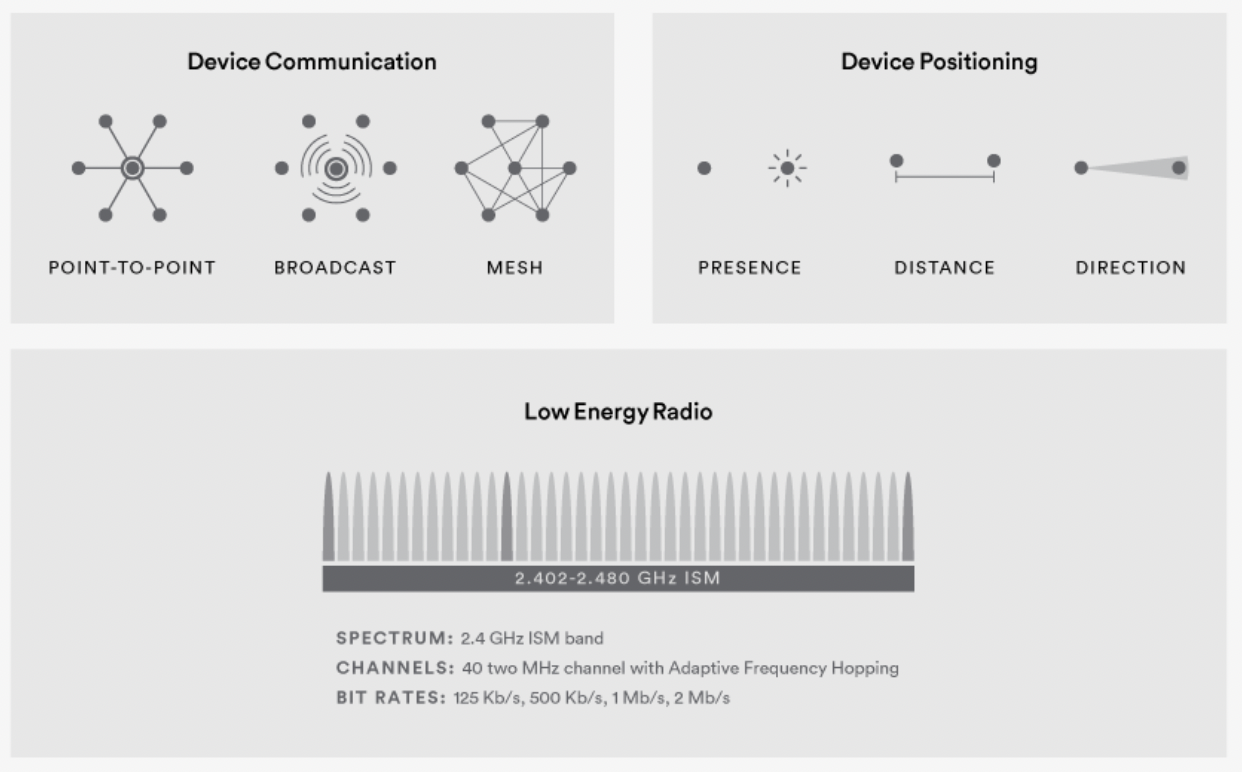
\includegraphics[width=1\textwidth]{images/ble.png}
    \caption{Bluetooth Low Energy specification; Source \autocite{bluetooth_tech_overview}}
\end{figure}